\chapter{Mediciones de Aplicaciones} \label{ch:measurements}

% **************************** Define Graphics Path **************************
\ifpdf
    \graphicspath{{Chapter5/Figs/Raster/}{Chapter5/Figs/PDF/}{Chapter5/Figs/}}
\else
    \graphicspath{{Chapter5/Figs/Vector/}{Chapter5/Figs/}}
\fi

En este capítulo se realizan diferentes tipos de mediciones de aplicación. El mismo se encuentra dividido en dos secciones, la primera trata sobre ensayos aplicados en el simulador, para estudiar el efecto de la utilización de un objeto externo para la medición de la distancia entre el radar y el objeto a medir. La segunda sección resume los resultados obtenidos de las mediciones tomadas con el radar sobre un portafolios metálico.


\section{Mediciones con Simulador}

En esta sección se realizan dos tipos de mediciones de aplicación con el simulador, representadas en la figura \ref{fig:DistDependencySim}. Se puede observar que la distancia entre el mezclador y el blanco es la distancia real sumada a un delta de distancia, el cual entre ensayo y ensayo se variará para obtener resultados. La primer medición toma al delta como valores conocidos, en cambio para la segunda, es tratada como una incertidumbre de medición.
\begin{figure}
  \centering
  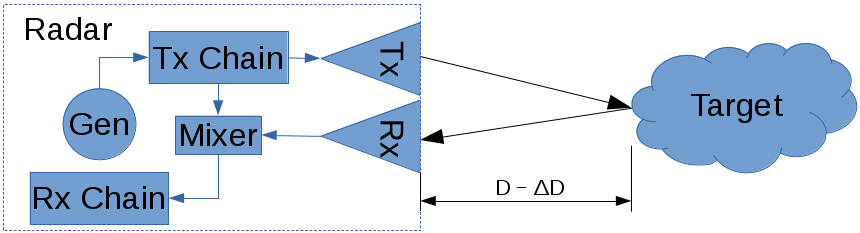
\includegraphics[width=12cm]{distanceDependency}
  \caption{Medición de propiedades del blanco ante diferentes deltas de distancias.}
  \label{fig:DistDependencySim}
\end{figure}


\subsection{Dependencia con distancia}

En esta sección se estudia la dependencia de la medición de los parámetros S del blanco iluminado con respecto a un error en la determinación de la distancia. Este ensayo es para determinar el efecto de utilizar un componente externo para medir el rango entre el blanco y el radar, y como el mismo no estaría en la posición del mezclador, se estaría introduciendo este tipo de error sistemático. 

La tabla \ref{tab:simDeltaDist} resume los resultados obtenidos. La columna Error indica el valor adoptado en la variable delta de la figura \ref{fig:DistDependencySim}. En otras palabras, sería a cuantos metros más cerca del blanco está el medidor de distancia con respecto al mezclador.

\begin{table}[htb]
  \caption{Parámetros S del blanco a distintas distancias utilizando el simulador.}
  \centering
  \label{tab:simDeltaDist}
  \begin{tabular}{l *{4}{S[table-auto-round, table-format=-1.2] S[table-auto-round, table-format=-3.2]}}
  \toprule
  \multirow{4}{1cm}{\textbf{Delta [m]}} & \multicolumn{8}{c}{\textbf{Distancia [m]}} \tabularnewline
  \cmidrule{2-9}
   & \multicolumn{2}{c}{30760} & \multicolumn{2}{c}{35000} & \multicolumn{2}{c}{37760,1695} & \multicolumn{2}{c}{40000} \tabularnewline
  \cmidrule(r){2-3} \cmidrule(lr){4-5} \cmidrule(lr){6-7} \cmidrule(l){8-9}
   & {Gain} & {Phase} & {Gain} & {Phase} & {Gain} & {Phase} & {Gain} & {Phase} \tabularnewline
   & [$\si{\deci\bel}$] & [$\si{\deg}$] & [$\si{\deci\bel}$] & [$\si{\deg}$] & [$\si{\deci\bel}$] & [$\si{\deg}$] & [$\si{\deci\bel}$] & [$\si{\deg}$] \tabularnewline
  \midrule
  
  0 & 0.9974998783 & -0.8999873159 & 0.9970854521 & 5.0829022535 & 0.9974244573 & 0.0563536612 & 0.9991246271 & 1.1021289469 \tabularnewline

  5 & 0.996851467 & -28.5141663823 & 0.9965158111 & -22.5305974732 & 0.9968962677 & -27.5567038267 & 0.9986251585 & -26.5105696718 \tabularnewline

  10 & 0.9962033718 & -56.1283462497 & 0.9959464141 & -50.1440980009 & 0.9963682879 & -55.1697621157 & 0.9981258771 & -54.1232690916 \tabularnewline

  40 & 0.9923214343 & 138.1865577226 & 0.9925351551 & 144.1748820091 & 0.9932048122 & 139.1518713272 & 0.9951341194 & 140.2005175668 \tabularnewline

  100 & 0.984591606 & 166.8162791476 & 0.9857389337 & 172.8127555094 & 0.986900466 & 167.7950516932 & 0.9891707856 & 168.8480043635 \tabularnewline

  \bottomrule 
  \end{tabular}
\end{table}

Se puede observar que la variación en el resultado para la determinación de la ganancia es despreciable, en cambio, para la fase es totalmente determinante. Cabe destacar que una separación entre el mezclador y el medidor de $\SI{5}{\meter}$ implica que la señal recorre $\SI{10}{\meter}$ menos, dado que la misma recorre el mismo camino dos veces. A su vez, independientemente de la distancia a la que está el blanco, un error igual a $\SI{5}{\meter}$ implica un desfase igual a $\SI{-27.61}{\deg}$. Este resultado es el esperado dado que la longitud de onda de la señal transmitida es aproximadamente $\SI{122}{\meter}$, por lo tanto un error de $\SI{12.2}{\meter}$ implica un desfase de $\SI{36}{\deg}$.

La figura \ref{fig:deltaDistSim} muestra de forma separada las mediciones de la ganancia y fase del blanco en las distancias $\SI{30760}{\meter}$, $\SI{35000}{\meter}$, $\SI{37760.1695}{\meter}$ y $\SI{40000}{\meter}$.
\begin{figure}[H]
  \centering
  \begin{subfigure}{0.49\textwidth}
    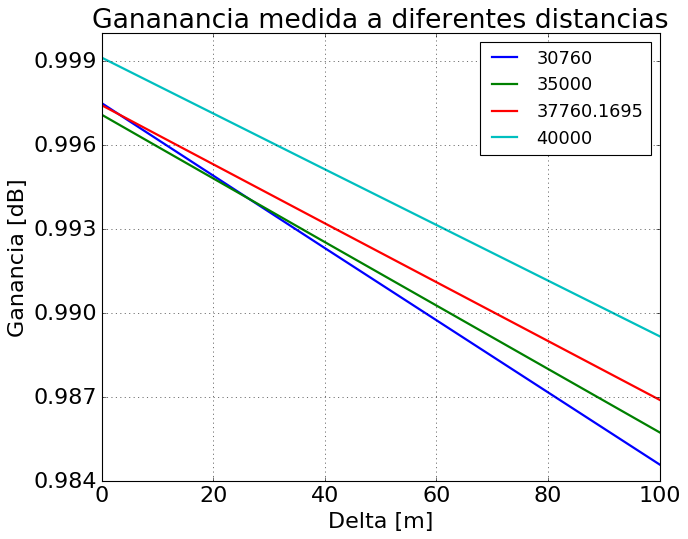
\includegraphics[width=7cm]{deltaDistGain}
    \caption{Ganancia}
  \end{subfigure}
  \begin{subfigure}{0.49\textwidth}
    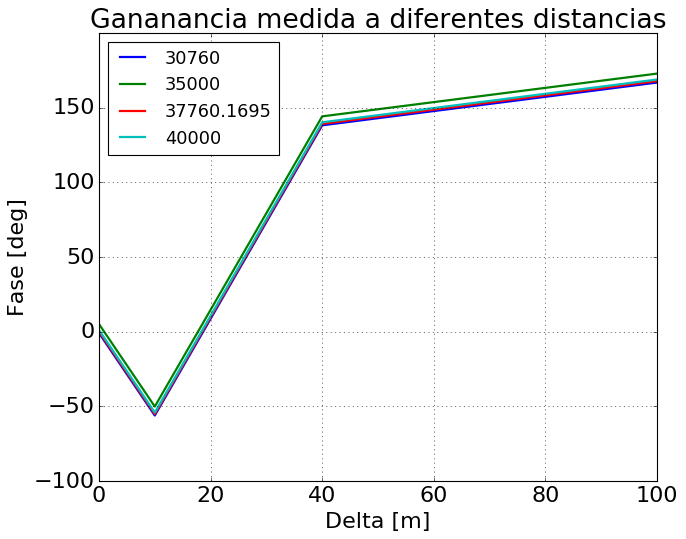
\includegraphics[width=7cm]{deltaDistPhase}
    \caption{Fase}
  \end{subfigure}
  \caption{Parámetros S del blanco a distintas distancias.}
  \label{fig:deltaDistSim}
\end{figure}

\subsection{Incertidumbre en distancia}

En esta sección se introducen incertidumbres en la medición de la distancia buscando determinar cómo afecta a la medición de los parámetros S del blanco iluminado. Dichas incertidumbres se las toma con distribución gaussiana con desvío estándar configurable y media igual a cero. La tabla \ref{tab:simIncertDist} resume los resultados obtenidos de la simulación de montecarlo con 1000 realizaciones.

\begin{table}[htb]
  \caption{Parámetros S del blanco a distintas distancias.}
  \centering
  \label{tab:simIncertDist}
  \begin{tabular}{l *{4}{S[table-auto-round, table-format=-1.2] S[table-auto-round, table-format=-3.2]}}
  \toprule
  \multirow{4}{1cm}{\textbf{Std [m]}} & \multicolumn{8}{c}{\textbf{Distancia [m]}} \tabularnewline
  \cmidrule{2-9}
   & \multicolumn{2}{c}{30760} & \multicolumn{2}{c}{35000} & \multicolumn{2}{c}{37760,1695} & \multicolumn{2}{c}{40000} \tabularnewline
  \cmidrule(r){2-3} \cmidrule(lr){4-5} \cmidrule(lr){6-7} \cmidrule(l){8-9}
   & {Gain} & {Phase} & {Gain} & {Phase} & {Gain} & {Phase} & {Gain} & {Phase} \tabularnewline
   & [$\si{\deci\bel}$] & [$\si{\deg}$] & [$\si{\deci\bel}$] & [$\si{\deg}$] & [$\si{\deci\bel}$] & [$\si{\deg}$] & [$\si{\deci\bel}$] & [$\si{\deg}$] \tabularnewline
  \midrule
  
  0 & 0.00 & 0.00 & 0.00 & 0.00 & 0.00 & 0.00 & 0.00 & 0.00 \tabularnewline

  5 & 0.000369507 & 15.7325843211 & 0.0003330912 & 16.1431290009 & 0.0002977873 & 15.5648756904 & 0.0002884168 & 15.9418570692 \tabularnewline

  10 & 0.0007337078 & 31.239336556 & 0.0006511433 & 31.5574962315 & 0.0006150956 & 32.1497974883 & 0.0005796089 & 32.0371315787 \tabularnewline

  40 & 0.0029849535 & 116.5644598149 & 0.002650077 & 116.673494049 & 0.0023426065 & 112.3447856255  & 0.0023238051 & 117.0437670382 \tabularnewline

  \bottomrule 
  \end{tabular}
\end{table}

Se puede observar que la variación en el resultado para la determinación de la ganancia es despreciable, en cambio, para la fase es totalmente determinante. Cabe destacar que la incertidumbre obtenida no depende de la distancia a la que se encuentra el blanco con respecto al radar.

La figura \ref{fig:incertDistSim} muestra la dependencia lineal entre la incertidumbre de la medición de la fase del blanco y el desvío estándar de la distancia al cual se encuentra. Se puede observar que si se desea no tener una incertidumbre absoluta mayor a $\SI{30}{\degree}$, no se debe tener una incertidumbre en la distancia mayor a $\SI{8.33}{\meter}$.
\begin{figure}[H]
  \centering
  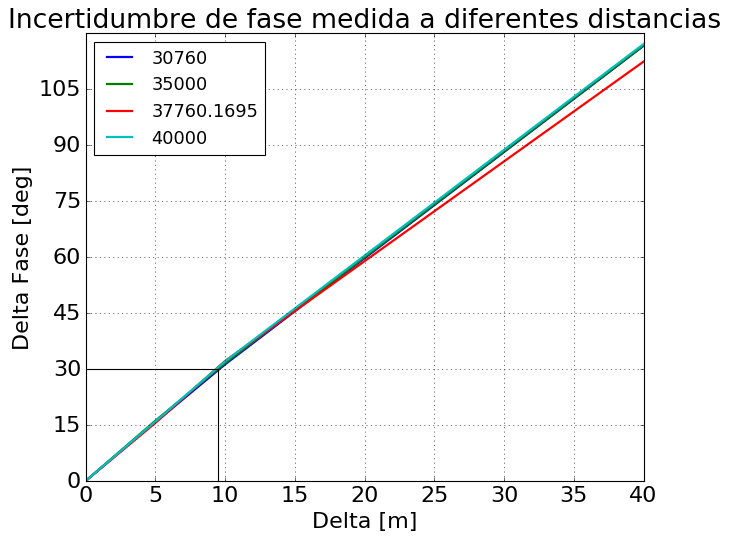
\includegraphics[width=9cm]{incertDistPhase}
  \caption{Medición de fase del blanco ante diferentes incertidumbres en distancias.}
  \label{fig:incertDistSim}
\end{figure}


\section{Mediciones con Radar}

En esta sección se realizan dos tipos de mediciones de aplicación con el radar utilizando como blanco a un portafolios frente a paneles absorvedores para disminuir los ecos en las paredes de la sala. El esquema de trabajo se encuentra representado en la figura \ref{fig:DistDependencySim2}. Se puede observar que la distancia entre el mezclador y el blanco es la distancia real sumada a un delta de distancia, el cual entre ensayo y ensayo, se variará para obtener resultados. Para la primer medición el delta es conocido, en cambio para la segunda, es tratado como una incertidumbre de medición y se lo mantuvo invariante.
% \begin{figure}[htb]
%   \centering
%   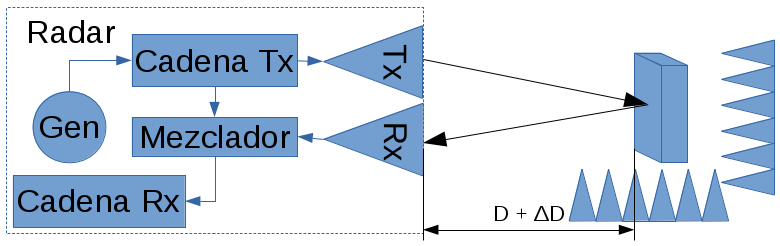
\includegraphics[width=12cm]{distanceDependencyRadar}
%   \caption{Medición de propiedades de un portafolios ante diferentes deltas de distancias.}
%   \label{fig:DistDependencySim2}
% \end{figure}

La figura \ref{fig:radarMeasurement} muestra el momento y el ambiente en que la medición tomó lugar.
\begin{figure}[htb]
  \centering
  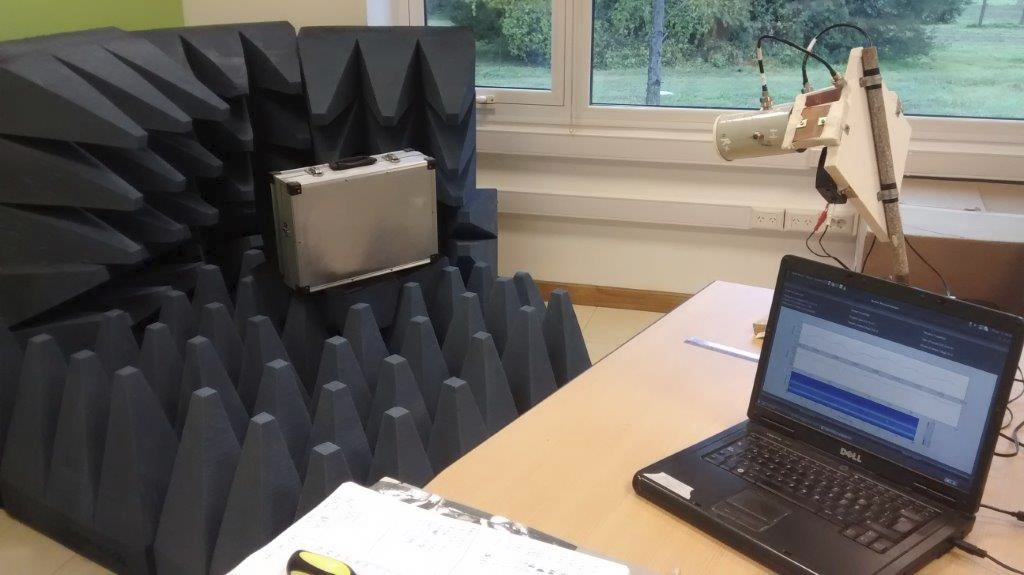
\includegraphics[width=12cm]{radarMeasurement}
  \caption{Medición de propiedades de un portafolios con el radar.}
  \label{fig:radarMeasurement}
\end{figure}


\subsection{Medición de un gabinete metálico}

En esta sección se realizan diferentes mediciones variando la distancia entre el gabinete y el radar. Para disminuir el eco recibido de las paredes que se encuentran detras del gabinete, se colocan paneles absorbedores. El objetivo de esta medición es la de determinar fuentes de incertidumbres que no se hayan tenido en cuenta previamente. La figura \ref{fig:DistDependencySim2} muestra el ambiente de trabajo.
\begin{figure}[htb]
  \centering
  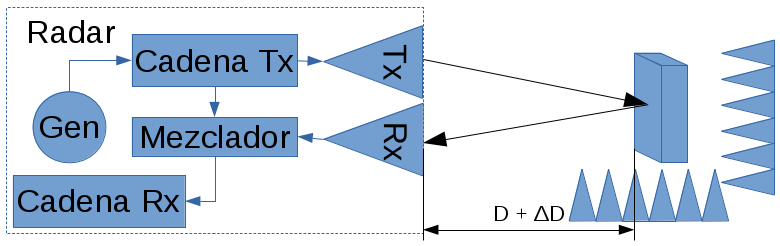
\includegraphics[width=12cm]{distanceDependencyRadar}
  \caption{Medición de propiedades de un gabinete metálico ante diferentes distancias.}
  \label{fig:DistDependencySim2}
\end{figure}

La tabla \ref{tab:radarMeasurementResults} resume los resultados obtenidos. El error absoluto en las mediciones equivale a tres veces el desvío estándar, dado que se toma como hipótesis la de estar trabajando con una incertidumbre con distribución gaussiana.

\begin{table}[H]
  \caption{Parámetros S del portafolios medidos con el radar.}
  \centering
  \label{tab:radarMeasurementResults}
  \begin{tabular}{c c | *{2}{S[table-auto-round, table-format=1.3]} *{2}{S[table-auto-round, table-format=-2.2]} S[table-auto-round, table-format=-3] S[table-auto-round, table-format=2]}
  \toprule
  \textbf{Rango} & \textbf{Pol} & \textbf{Rango} & \textbf{$\Delta$Rango}  & \textbf{Gain} & \textbf{$\Delta$Gain} & \textbf{Phase} & \textbf{$\Delta$Phase} \tabularnewline

  [$\si{\meter}$] & & [$\si{\meter}$] & [$\si{\meter}$] & [$\si{\dB}$] & [$\si{\dB}$] & [$\si{\deg}$] & [$\si{\deg}$] \tabularnewline
  \midrule
  
  \multirow{4}{*}{1.32} & HH & 2.201 & 0.013 & 31.4539 & 0.0915 & 4.5 & 69.8 \tabularnewline
   & HV & 2.204 & 0.015 & 22.9796 & 0.1261 & -131.1 & 81.0 \tabularnewline
   & VH & 2.425 & 0.023 & 25.3829 & 0.2481 & -140.8 & 80.4 \tabularnewline
   & VV & 1.399 & 0.007 & 17.0184 & 0.1307 & 97.1 & 37.2 \tabularnewline

  \cmidrule{2-8}
  \multirow{4}{*}{1.56} & HH & 1.572 & 0.005 & 24.4271 & 0.0654 & -118.9 & 30.0 \tabularnewline
   & HV & 1.738 & 0.008 & 18.8475 & 0.0839 & -78.8 & 42.0 \tabularnewline
   & VH & 1.338 & 0.007 & 12.3065 & 0.0954 & 30.5 & 39.7 \tabularnewline
   & VV & 1.630 & 0.006 & 22.9165 & 0.1030 & -102.1 & 37.1 \tabularnewline

  \cmidrule{2-8}
  \multirow{4}{*}{1.71} & HH & 1.709 & 0.006 & 26.4757 & 0.0651 & 174.5 & 31.9 \tabularnewline
   & HV & 2.929 & 0.004 & 23.9049 & 0.0759 & -65.9 & 19.6 \tabularnewline
   & VH & 2.343 & 0.007 & 22.0027 & 0.0613 & -99.0 & 36.5 \tabularnewline
   & VV & 1.685 & 0.008 & 22.982 & 0.1295 & 58.9 & 49.5 \tabularnewline

  \cmidrule{2-8}
  \multirow{4}{*}{1.84} & HH & 1.994 & 0.006 & 28.0666 & 0.0532 & -90.1 & 33.6 \tabularnewline
   & HV & 1.224 & 0.007 & 5.9869 & 0.1663 & -61.1 & 40.2 \tabularnewline
   & VH & 2.258 & 0.006 & 18.3366 & 0.0649 & -1.3 & 31.9 \tabularnewline
   & VV & 2.072 & 0.003 & 26.4441 & 0.0632 & -73.7 & 22.2 \tabularnewline

  \cmidrule{2-8}
  \multirow{4}{*}{2.005} & HH & 2.364 & 0.008 & 30.0745 & 0.0695 & -190.8 & 43.1 \tabularnewline
   & HV & 3.896 & 0.013 & 25.8801 & 0.1221 & 10.7 & 71.8 \tabularnewline
   & VH & 2.259 & 0.006 & 18.1211 & 0.0513 & -7.8 & 35.5 \tabularnewline
   & VV & 2.108 & 0.005 & 24.5758 & 0.0572 & 15.0 & 28.8 \tabularnewline

  \bottomrule
  \end{tabular}
\end{table}

Analizando los resultados obtenidos en la tabla \ref{tab:radarMeasurementResults}, se pueden obtener las siguientes conclusiones:
\begin{description}
  \item[Determinación distancia] Se puede observar que se determina erróneamente la distancia al blanco. Esto se debe a que no se realizó una medición previa del clutter de la sala para substraer dicho efecto. En la figura \ref{fig:distanceError} se observa la FFT de la señal recibida, en la cual se indica que la potencia de la señal que se corresponde al eco del blanco es menor que la del propio clutter. De esta forma, se determina de una forma errónea la distancia al blanco.

  A su vez, se observa que sistemáticamente la ganancia para la polarización HH es mayor que para el resto. Dicho comportamiento se debe a que el crosstalk entre las antenas para dicha combinación de polarizaciones es la máxima medida, ver \ref{ssc:sParameters}.

  \begin{figure}[htb]
    \centering
    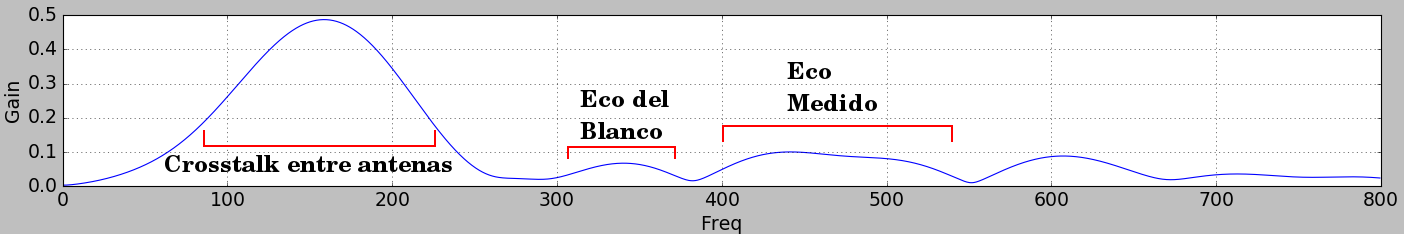
\includegraphics[width=15cm]{distanceError}
    \caption{FFT del eco recibido por el radar. Se observa que la potencia del eco recibido por el blanco es menor que el del clutter.}
    \label{fig:distanceError}
  \end{figure}

  \item[Determinación de Ganancia] Se puede observar que se determina erróneamente la relación de ganancia entre la señal incidente y reflejada del blanco. Esto se debe a tres causas principales. La primera se debe a que, como se mide de forma incorrecta la distancia al blanco, la atenuación real que impone el medio sobre la señal no es la calculada. La segunda está relacionada a que no se tomó en cuenta que el control del volumen de la computadora estaba en modo automático, por lo tanto entre ensayo y ensayo se modificó el nivel de la señal recibida, introduciendo un error grosero en dicha magnitud. La tercera se debe a que, como se puede observar en la figura \ref{fig:distanceError}, los niveles de potencia de la señal recibida son principalmente del clutter del ambiente. La mejor solución de este problema es la de realizar una medición previa del clutter sin blanco para realizar la resta de señales.

  \item[Determinación de Fase] Se puede observar que se determina erróneamente la relación de fase entre la señal incidente y reflejada del blanco. Esto es debe a dos causas principales. La primera se debe a que, como se mide de forma incorrecta la distancia al blanco, el desfase real que impone el medio sobre la señal no es la calculada. La segunda se debe a que, como no se eliminó el clutter de la señal, la medición resulta afectada.
\end{description}


\subsection{Dependencia con distancia}

En esta sección se estudia la dependencia de la medición de los parámetros S del blanco iluminado con respecto a un error en la determinación de la distancia. Este ensayo es para determinar el efecto de utilizar un componente externo para medir el rango entre el blanco y el radar, y como el mismo no estaría en la posición del mezclador, se estaría introduciendo este tipo de error sistemático.

La tabla \ref{tab:simDeltaDistRadar} resume los resultados obtenidos. La columna Error indica el valor adoptado en la variable delta de la figura \ref{fig:DistDependencySim2}. En otras palabras, sería a cuantos metros más cerca del blanco está el medidor de distancia con respecto al mezclador.

\begin{table}[htb]
  \caption{Parámetros S del blanco a distintas distancias utilizando el radar.}
  \centering
  \label{tab:simDeltaDistRadar}
  \begin{tabular}{l *{3}{S[table-auto-round, table-format=-1.2] S[table-auto-round, table-format=-3.2]}}
  \toprule
  \multirow{4}{1cm}{\textbf{Delta [$\si{\milli\meter}$]}} & \multicolumn{6}{c}{\textbf{Distancia [$\si{\meter}$]}} \tabularnewline
  \cmidrule{2-7}
   & \multicolumn{2}{c}{1,71} & \multicolumn{2}{c}{1,84} & \multicolumn{2}{c}{2,005} \tabularnewline
  \cmidrule(r){2-3} \cmidrule(lr){4-5} \cmidrule(l){6-7}
   & {Gain} & {Phase} & {Gain} & {Phase} & {Gain} & {Phase} \tabularnewline
   & [$\si{\dB}$] & [$\si{\deg}$] & [$\si{\dB}$] & [$\si{\deg}$] & [$\si{\dB}$] & [$\si{\deg}$] \tabularnewline
  \midrule
  
  0 & 81.464 & -174.1 & 81.654 & 57.2 & 82.18 & 5 \tabularnewline

  5 & 80.947 & 100.3 & 81.175 & -28.4 & 82.14 & 32.4 \tabularnewline

  10 & 80.417 & 14.7 & 80.677 & -114 & 82.104 & 60 \tabularnewline

  15 & 79.873 & -70.9 & 80.17 & 160.3 & 82.063 & 87.4 \tabularnewline

  \bottomrule 
  \end{tabular}
\end{table}
\todo[inline]{actualizar la tabla a algo posta}
Se puede observar que la variación en el resultado para la determinación de la ganancia no resulta despreciable dado que al haber $\SI{15}{\milli\meter}$ de diferencia la medición disminuyó en $\SI{1.591}{\dB}$ y para el caso de la fase es totalmente determinante. Cabe destacar que una separación entre el mezclador y el medidor de $\SI{5}{\milli\meter}$ implica que la señal recorre $\SI{10}{\milli\meter}$ menos, dado que la misma recorre el mismo camino dos veces. A su vez, independientemente de la distancia a la que está el blanco, un error igual a $\SI{5}{\milli\meter}$ implica un desfase igual a $\SI{27.6}{\deg}$. Este resultado es el esperado dado que la longitud de onda de la señal transmitida es aproximadamente $\SI{122}{\milli\meter}$, por lo tanto un error de $\SI{12.2}{\meter}$ implica un desfase de $\SI{36}{\deg}$.

\begin{figure}[H]
  \centering
  \begin{subfigure}{0.49\textwidth}
    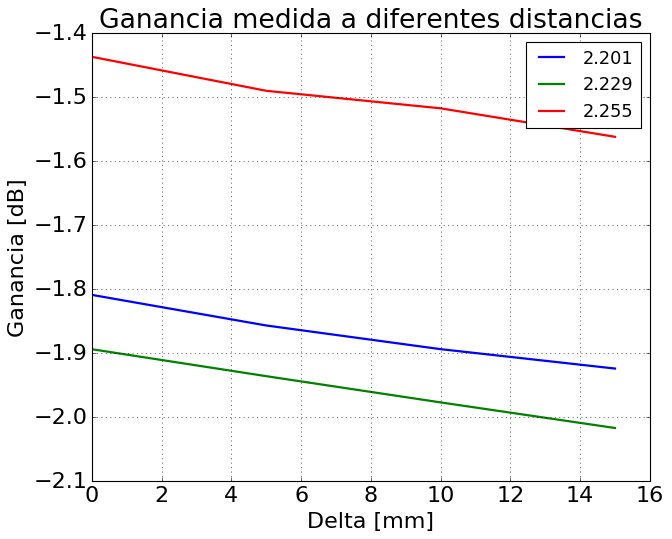
\includegraphics[width=7cm]{deltaDistGainRadar}
    \caption{Ganancia}
  \end{subfigure}
  \begin{subfigure}{0.49\textwidth}
    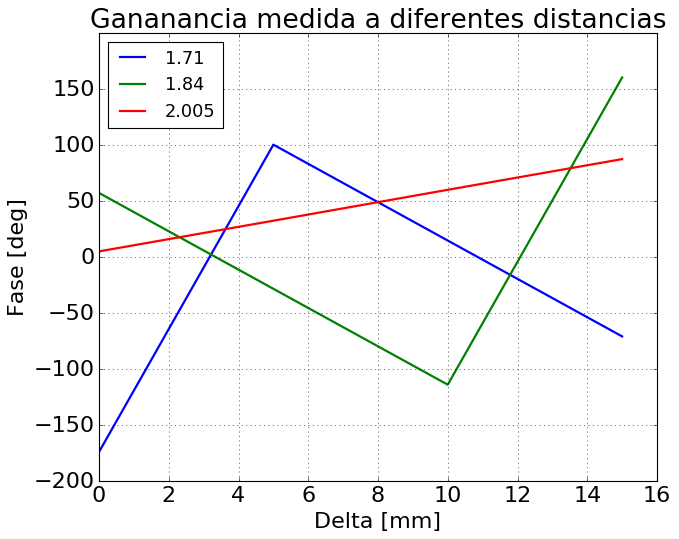
\includegraphics[width=7cm]{deltaDistPhaseRadar}
    \caption{Fase}
  \end{subfigure}
  \caption{Parámetros S del blanco a distintas distancias.}
  \label{fig:deltaDistRadar}
\end{figure}
La figura \ref{fig:deltaDistRadar} muestra de forma separada las mediciones de la ganancia y fase del blanco en las distancias $\SI{1.71}{\meter}$, $\SI{1.84}{\meter}$ y $\SI{2.005}{\meter}$. Se puede observar que para las distancias menores la variación de ganancia es mucho mayor que a la máxima medida, esto se atribuye a una mayor influencia de los lóbulos secundarios del crosstalk sobre las mismas. Se puede apreciar lo mismo ante la variación de fase.


\subsection{Incertidumbre en Distancia}
\todo[inline]{hacer}

\subsection{Mediciones a diferentes distancias}

En esta sección se realizan diferentes mediciones variando la distancia al cuerpo para ver si hay variaciones en la determinación de los parámetros S del blanco iluminado. Se escojen dos tipos de blancos, un maletin y un corner reflector.


\subsubsection{Medición de un Corner Reflector}

Para esta experiencia se construye un corner reflector triangular de $\SI{50}{\centi\meter}$ de lado, ver figura \ref{fig:corner}. El máximo RCS que se puede obtener, siguiendo la ecuación \ref{eq:theoreticalRcs}, es igual a $\SI{12.43}{\dB}$. % Luego de su construcción, se midieron el ángulo de cada cara y se observa que poseen $\SI{88.5}{\deg}$, esto implica que el eco recibido debería estar disminuído en $\SI{10}{\dB}$, ver figura \ref{fig:cornerErrors}.
\begin{figure}[htb]
  \centering
  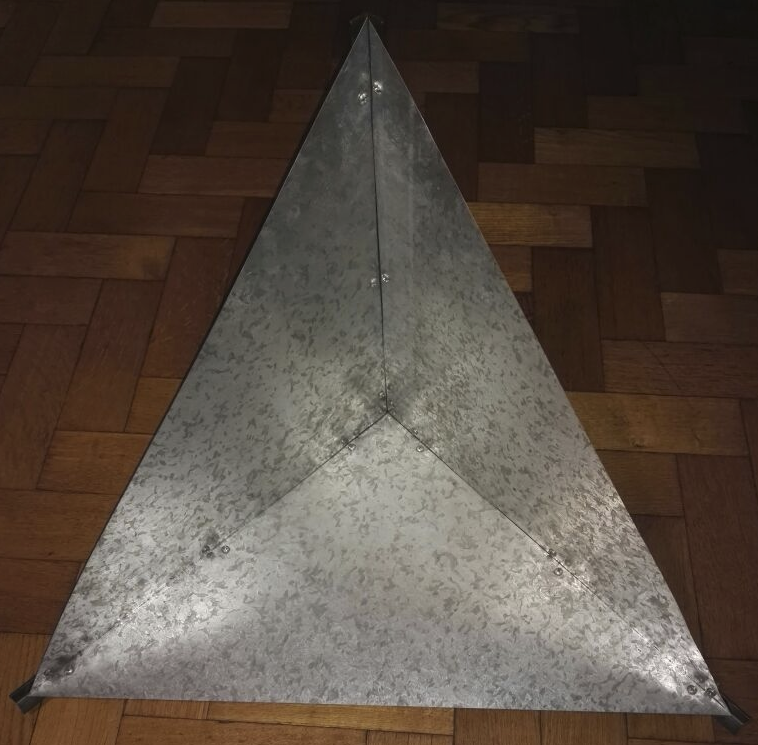
\includegraphics[width=6cm]{cornerReflector}
  \caption{Corner reflector construído de $\SI{50}{\centi\meter}$ de lado para realizar las mediciones.}
  \label{fig:corner}
\end{figure}

La disposición del radar y del corner reflector en la sala se muestra en la figura \ref{fig:cornerReflectorMeasurement}. Se puede determinar que el ángulo de incidencia con respecto a la horizontal resulta del orden de $\SI{24}{\deg}$. Por lo tanto, se espera una disminución de $\SI{3}{\dB}$, la cual se determina en la figura \ref{fig:cornerRel}. A su vez, en la figura \ref{fig:cornerErrors} se muestra cómo el RCS resulta afectado ante la pérdida de ortogonalidad entre las caras del corner. Se espera que haya una pérdida extra del orden de los $\SI{10}{\dB}$.

La tabla \ref{tab:cornerMeasurementResults} resume los resultados obtenidos. El error absoluto en las mediciones equivale a tres veces el desvío estándar, dado que se toma como hipótesis la de estar trabajando con una incertidumbre con distribución gaussiana.

\begin{table}[H]
  \caption{Parámetros de dispersión del corner reflector medidos con el radar.}
  \centering
  \label{tab:cornerMeasurementResults}
  \begin{tabular}{c c | S[table-auto-round, table-format=1.2] S[table-auto-round, table-format=1.2] S[table-auto-round, table-format=-2.2] S[table-auto-round, table-format=1.2] S[table-auto-round, table-format=-3] S[table-auto-round, table-format=2]}
  \toprule
  \textbf{Rango} & \textbf{Pol} & \textbf{Rango} & \textbf{$\Delta$Rango}  & \textbf{Gain} & \textbf{$\Delta$Gain} & \textbf{Phase} & \textbf{$\Delta$Phase} \tabularnewline

  [$\si{\meter}$] & & [$\si{\meter}$] & [$\si{\meter}$] & [$\si{\dB}$] & [$\si{\dB}$] & [$\si{\deg}$] & [$\si{\deg}$] \tabularnewline
  \midrule

  \multirow{4}{*}{2,201} & HH & 2.201 & 0.011 & 1.3969 & 1.1 & -24.1 & 26.1 \tabularnewline
   & HV & 2.247 & 0.026 & -14.0225 & 1.5631 & -73.1 & 13.9 \tabularnewline
   & VH & 2.288 & 0.036 & -14.1252 & 2.1342 & -92.4 & 87.1 \tabularnewline
   & VV & 2.195 & 0.014 & -1.8092 & 0.3614 & 147.7 & 7.3 \tabularnewline

  \cmidrule{2-8}
  \multirow{4}{*}{2,229} & HH & 2.223 & 0.017 & 1.2961 & 1.0128 & -11.0 & 9.3 \tabularnewline
   & HV & 2.313 & 0.041 & -13.3133 & 1.5806 & -71.5 & 14.0 \tabularnewline
   & VH & 2.317 & 0.038 & -14.7132 & 2.3655 & -93.3 & 87.3 \tabularnewline
   & VV & 2.246 & 0.023 & -1.8941 & 0.2935 & 133.2 & 12.3 \tabularnewline

  \cmidrule{2-8}
  \multirow{4}{*}{2,255} & HH & 2.26 & 0.01 & 1.6825 & 0.4407 & -4.0 & 5.2 \tabularnewline
   & HV & 2.305 & 0.038 & -14.2542 & 1.2031 & -59.7 & 18.3 \tabularnewline
   & VH & 2.359 & 0.049 & -13.4975 & 1.8296 & -95.4 & 33.8 \tabularnewline
   & VV & 2.245 & 0.019 & -1.4372 & 0.3531 & 152.1 & 7.8 \tabularnewline

  \cmidrule{2-8}
  \multirow{4}{*}{2,285} & HH & 2.272 & 0.021 & 1.9684 & 1.0278 & -3.23 & 9.9 \tabularnewline
   & HV & 2.398 & 0.039 & -14.3538 & 1.1613 & -83.6 & 16.9 \tabularnewline
   & VH & 2.379 & 0.052 & -14.1736 & 1.5638 & -95.2 & 60.2 \tabularnewline
   & VV & 2.287 & 0.023 & -1.6621 & 0.3498 & 177.4 & 12.4 \tabularnewline

  \bottomrule
  \end{tabular}
\end{table}

Las figuras \ref{fig:measuredDistCorner}, \ref{fig:measuredGainCorner} y \ref{fig:measuredPhaseCorner} muestran las distancias, ganancias y desfases esperados y medidos por le radar asociados a sus respectivas incertidumbres con respecto a las distintas distancias medidas con una cinta métrica. Se puede concluir lo siguiente:
\begin{figure}[H]
  \centering
  \begin{subfigure}{0.49\textwidth}
    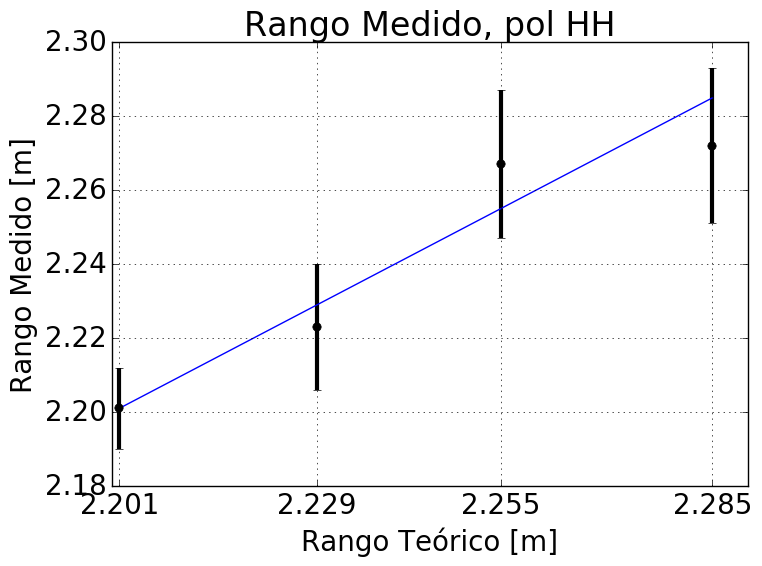
\includegraphics[width=6cm]{measuredCornerRangeHH}
  \end{subfigure}
  \begin{subfigure}{0.49\textwidth}
    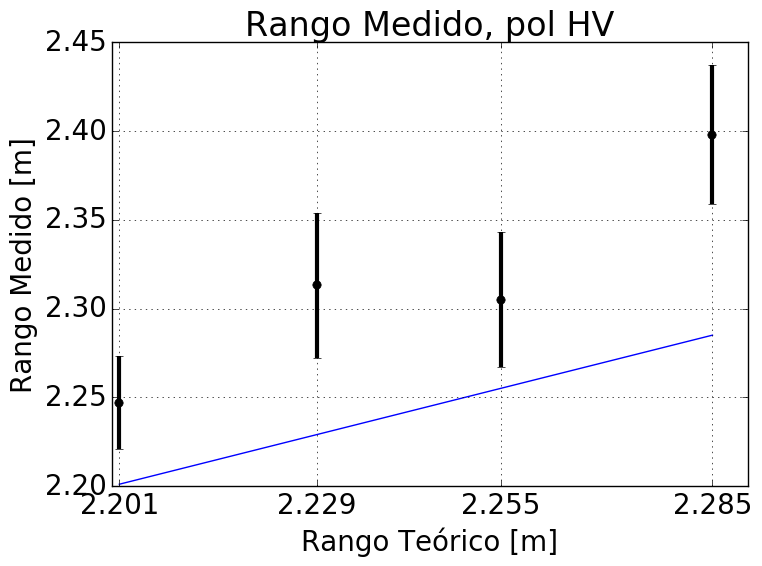
\includegraphics[width=6cm]{measuredCornerRangeHV}
  \end{subfigure}

  \begin{subfigure}{0.49\textwidth}
    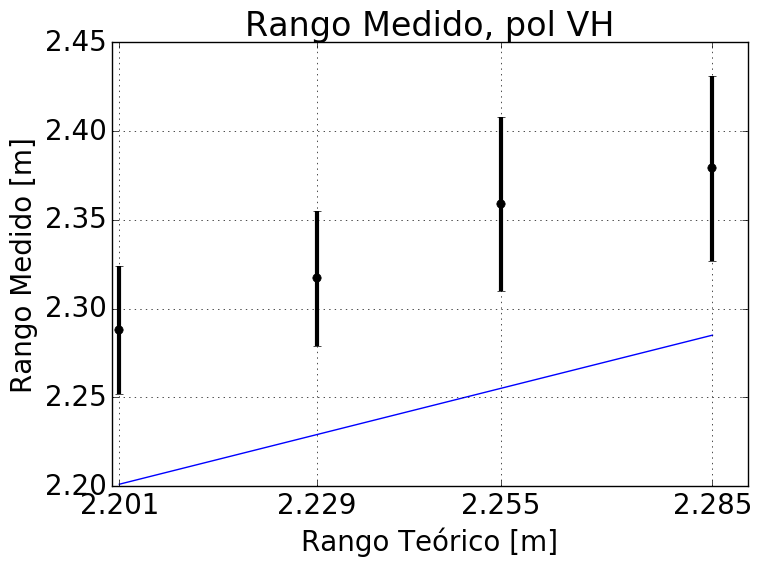
\includegraphics[width=6cm]{measuredCornerRangeVH}
  \end{subfigure}
  \begin{subfigure}{0.49\textwidth}
    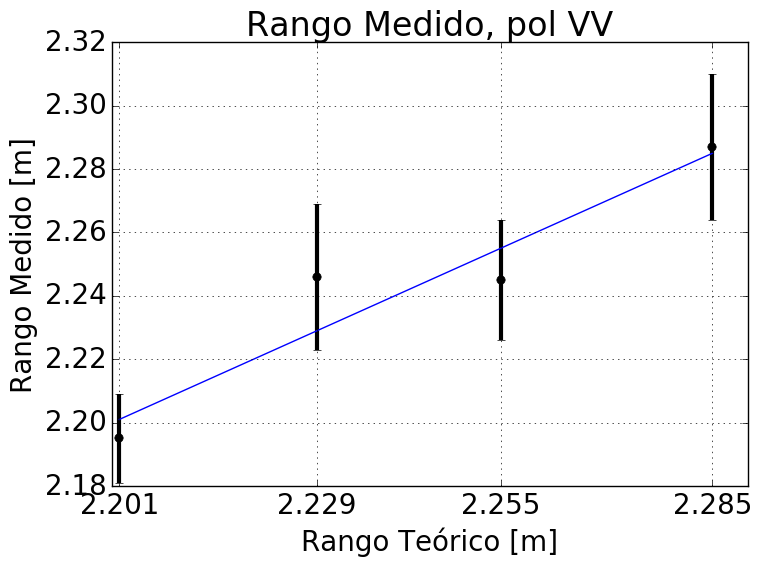
\includegraphics[width=6cm]{measuredCornerRangeVV}
  \end{subfigure}
  \caption{Distancia medida con su incertidumbre por el radar con respecto a la distancia medida con una cinta métrica.}
  \label{fig:measuredDistCorner}
\end{figure}
\begin{figure}[H]
  \centering
  \begin{subfigure}{0.49\textwidth}
    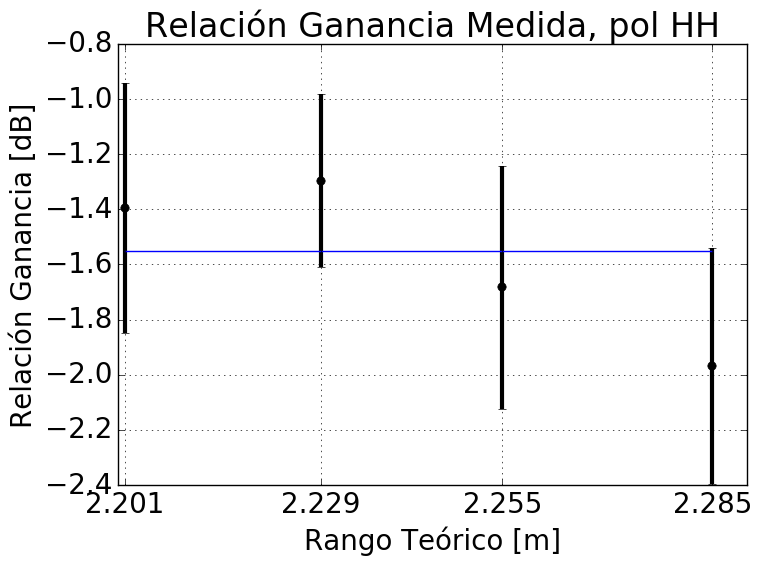
\includegraphics[width=6cm]{measuredCornerGainHH}
  \end{subfigure}
  \begin{subfigure}{0.49\textwidth}
    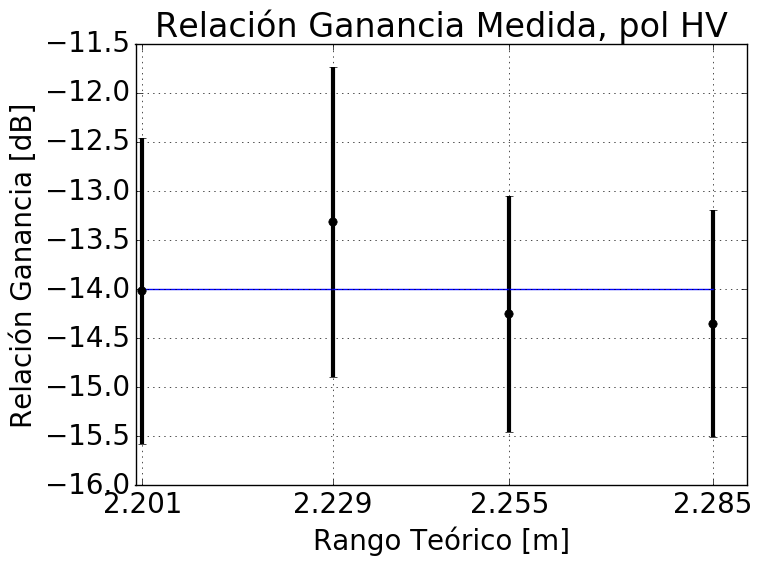
\includegraphics[width=6cm]{measuredCornerGainHV}
  \end{subfigure}

  \begin{subfigure}{0.49\textwidth}
    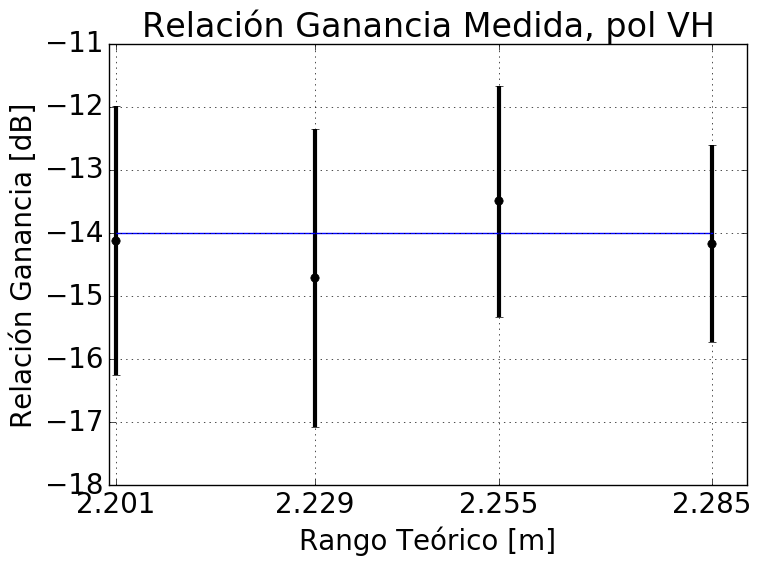
\includegraphics[width=6cm]{measuredCornerGainVH}
  \end{subfigure}
  \begin{subfigure}{0.49\textwidth}
    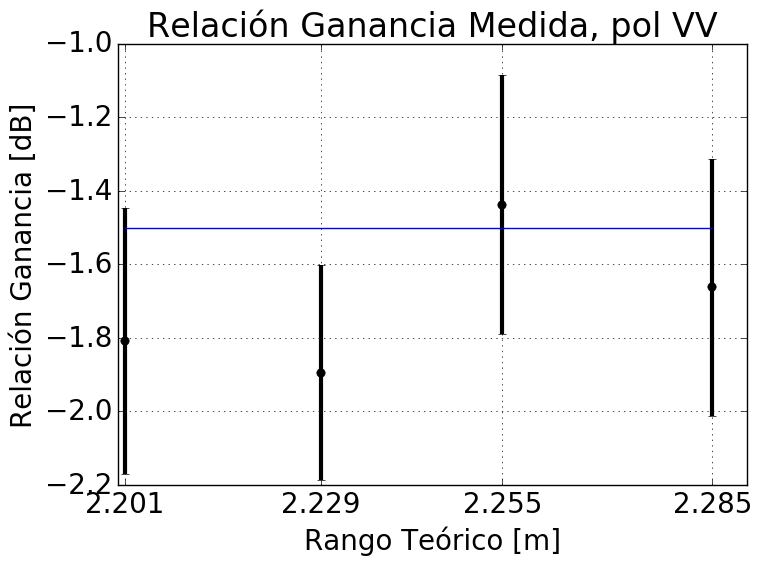
\includegraphics[width=6cm]{measuredCornerGainVV}
  \end{subfigure}
  \caption{Ganancia medida del blanco con su incertidumbre por el radar con respecto a la distancia medida con una cinta métrica.}
  \label{fig:measuredGainCorner}
\end{figure}
\begin{figure}[H]
  \centering
  \begin{subfigure}{0.49\textwidth}
    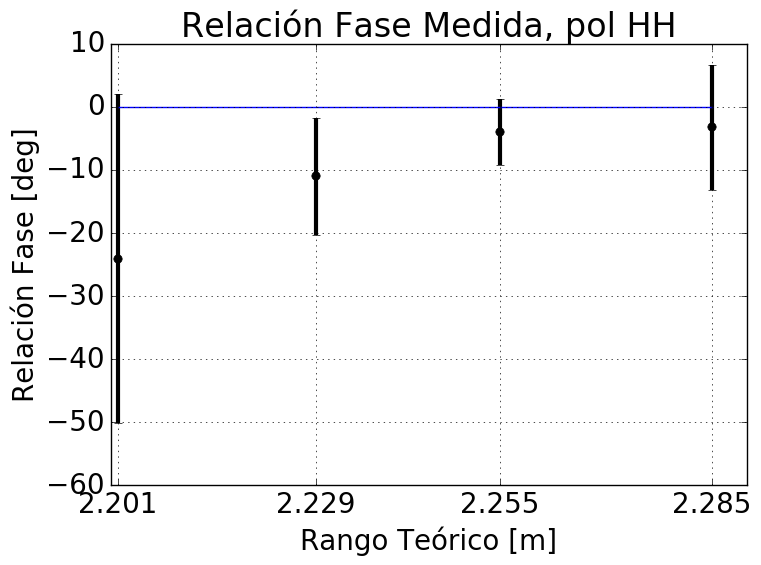
\includegraphics[width=6cm]{measuredCornerPhaseHH}
  \end{subfigure}
  \begin{subfigure}{0.49\textwidth}
    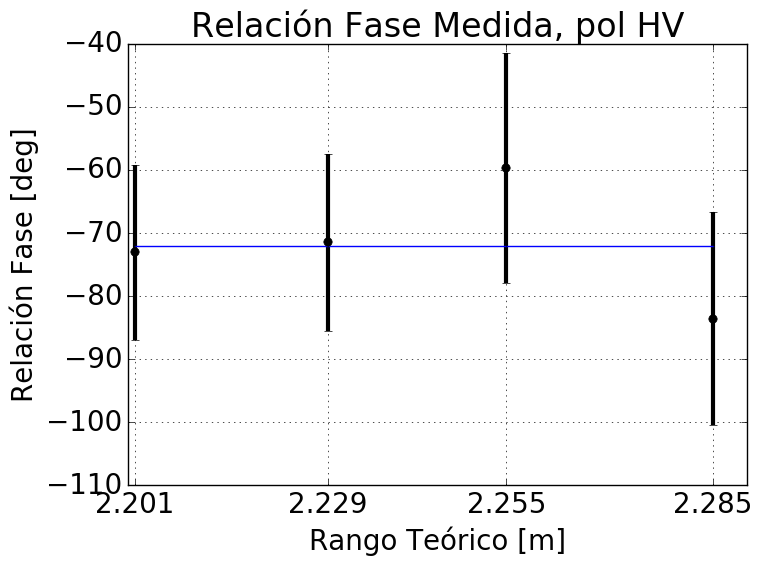
\includegraphics[width=6cm]{measuredCornerPhaseHV}
  \end{subfigure}

  \begin{subfigure}{0.49\textwidth}
    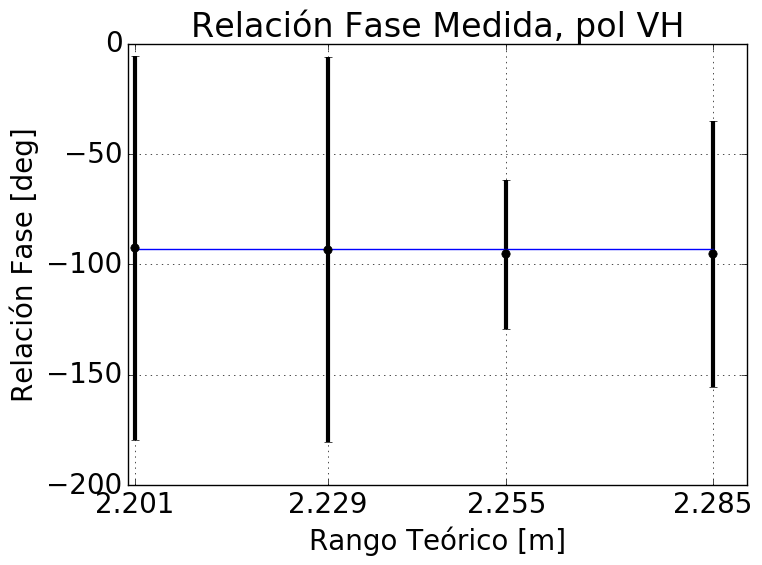
\includegraphics[width=6cm]{measuredCornerPhaseVH}
  \end{subfigure}
  \begin{subfigure}{0.49\textwidth}
    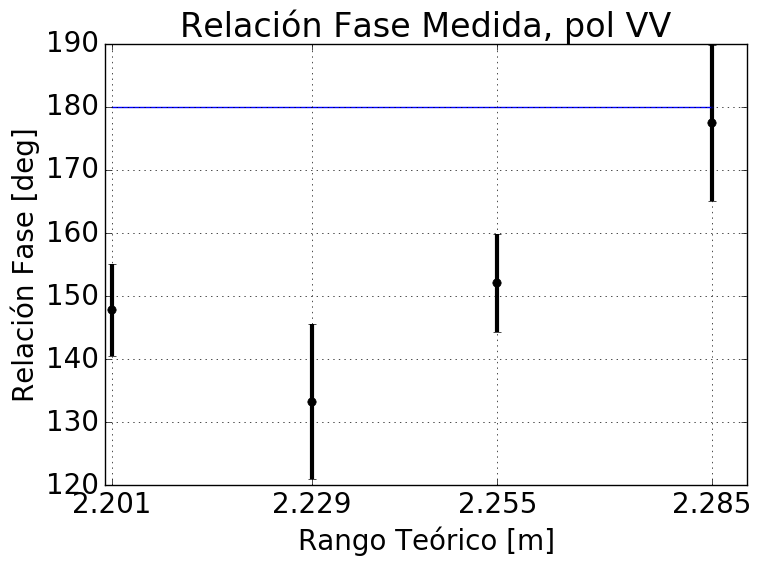
\includegraphics[width=6cm]{measuredCornerPhaseVV}
  \end{subfigure}
  \caption{Fase medida del blanco con su incertidumbre por el radar con respecto a la distancia medida con una cinta métrica.}
  \label{fig:measuredPhaseCorner}
\end{figure}


\begin{description}
  \item[Determinación distancia] Se puede observar que el radar determina correctamente la distancia al blanco para las adquisiciones co-polares. En cambio, como el corner posee un alto rechazo para adquisiciones cross-polares, el radar detecta la presencia de otro cuerpo de la sala en que se realizaron las mediciones. Hay algunas adquisiciones co-polares en donde la distancia indicada por el radar es un par de cenímetros mayor al ideal, esto se debe a que entre adquisiciones el blanco fue removido y vuelto a colocar sin volver a medir que el mismo quede exactamente en la misma posición. En la figura \ref{fig:correctDistance} se muestra la FFT de la señal recibida con el blanco luego de haber eliminado el clutter.

  \begin{figure}[htb]
    \centering
    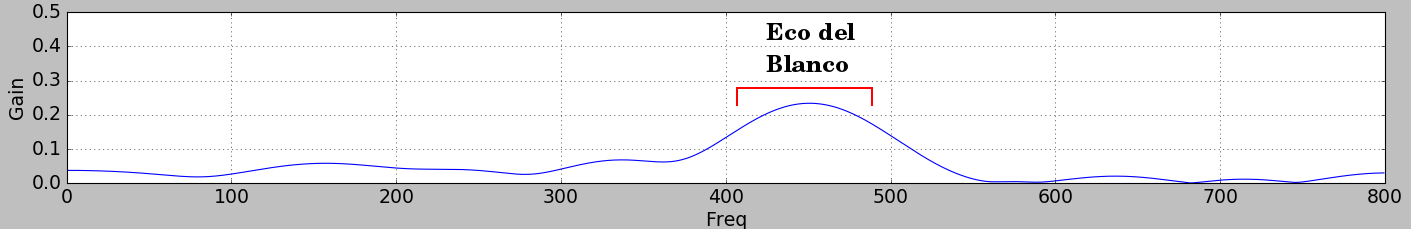
\includegraphics[width=15cm]{correctDistance}
    \caption{FFT del eco recibido por el radar. Se observa que la potencia del eco recibido por el blanco es mayor que el del clutter.}
    \label{fig:correctDistance}
  \end{figure}

  \item[Determinación de Ganancia] Se puede observar que el radar detecta correctamente las ganancias del corner reflector. Se aprecia una disminución de $\SI{14}{\dB}$ para adquisiciones cross-polares con respecto a las co-polares. A su vez, se puede apreciar que la adquisición con polarización VV posee unos $\SI{2}{\dB}$ menos que con polarización HH. Esto se debe a se atribuye a errores en la construcción del corner reflector. \todo[inline]{terminar :D }

  \item[Determinación de Fase] Se puede observar que se determina erróneamente la relación de fase entre la señal incidente y reflejada del blanco. Esto es debe a dos causas principales. La primera se debe a que, como se mide de forma incorrecta la distancia al blanco, el desfase real que impone el medio sobre la señal no es la calculada. La segunda se debe a que, como no se eliminó el clutter de la señal, la medición resulta afectada.
\end{description}



\section{Resumen}

En este capítulo se realizaron mediciones de aplicación tanto con el simulador como con el radar.

Con el simulador se estudió la dependencia del resultado ante errores en la determinación de la distancia y ante incertidumbres en la misma. Para el primer caso la determinación de la ganancia es casi invariante, en cambio para la fase se puede observar que ante diferencias de distancia de $\lambda / 10$ se observan desfases de $\SI{36}{\degree}$. Para el segundo caso, se repiten los mismos resultados dado que si se desea tener una incertidumbre menor a $\SI{36}{\degree}$, se debe tener una incertidumbre menor a $\lambda / 10$ en la determinación de la distancia.

Con el radar se realizaron ensayos de la dependencia del resultado ante errores en la determinación de la distancia y se midió de mismo blanco a distintas distancias. Para el primer caso, solamente se observa el resultado esperado en la determinación de la ganancia y fase para una distancia mínima de $\SI{2}{\meter}$, para distancias menores se debe evitar realizar mediciones dado que los lóbulos secundarios del cross-talk entre las antenas interfieren la medición.